%%%%%%%%%%%%%%%%%%%%% chapter.tex %%%%%%%%%%%%%%%%%%%%%%%%%%%%%%%%%
%
% sample chapter
%
% Use this file as a template for your own input.
%
%%%%%%%%%%%%%%%%%%%%%%%% Springer-Verlag %%%%%%%%%%%%%%%%%%%%%%%%%%
%\motto{Use the template \emph{chapter.tex} to style the various elements of your chapter content.}

\chapter{Rosetta Code Tasks starting with N}

\section*{N-queens problem}

Solve the
\href{http://en.wikipedia.org/wiki/Eight\_queens\_puzzle}{eight queens
  puzzle}. You can extend the problem to solve the puzzle with a board
of side NxN.

Cf.

\begin{itemize}
\item
  \emph{Knight's tour}
\end{itemize}



\begin{wideverbatim}

(load "@lib/simul.l")

(de queens (N)
   (let (R (range 1 N)  Cnt 0)
      (for L (permute (range 1 N))
         (when
            (= N
               (length (uniq (mapcar + L R)))
               (length (uniq (mapcar - L R))) )
            (inc 'Cnt) ) )
      Cnt ) )

This alternative version does not first pre-generate all permutations with
'permute', but creates them recursively. Also, it directly checks for
duplicates, instead of calling 'uniq' and 'length'. This is much faster.

(de queens (N)
   (let (R (range 1 N)  L (copy R)  X L  Cnt 0)
      (recur (X)  # Permute
         (if (cdr X)
            (do (length X)
               (recurse (cdr X))
               (rot X) )
            (or
               (seek  # Direct check for duplicates
                  '((L) (member (car L) (cdr L)))
                  (mapcar + L R) )
               (seek
                  '((L) (member (car L) (cdr L)))
                  (mapcar - L R) )
               (inc 'Cnt) ) ) )
      Cnt ) )

Output in both cases:

: (queens 8)
-> 92

\end{wideverbatim}

\pagebreak{}
\section*{Named parameters}

Create a function which takes in a number of arguments which are
specified by name rather than (necessarily) position, and show how to
call the function. If the language supports reordering the arguments or
optionally omitting some of them, note this.

\textbf{Note:}

Named parameters relies on being able to use the names given to function
parameters when the function is defined, when assigning arguments when
the function is called.

For example, if f a function were to be defined as 

\begin{verbatim}
  define func1 (paramname1, paramname2); 
\end{verbatim}

then it could be called normally as

\begin{verbatim}
  func1(argument1, argument2)
\end{verbatim}

and in the called function paramname1 would be associated with
argument1 and paramname2 with argument2.

\texttt{func1} \textbf{must also be able to be called in a way that
visually binds each parameter to its respective argument, irrespective
of argument order}, for example:

\begin{verbatim}
  func1(paramname2=argument2, paramname1=argument1)
\end{verbatim}

which \emph{explicitly} makes the same parameter/argument bindings as
before.

Named parameters are often a feature of languages used in safety
critical areas such as
\href{http://en.wikipedia.org/wiki/Verilog}{Verilog} and
\href{http://en.wikipedia.org/wiki/VHDL}{VHDL}.

\textbf{See also:}

\begin{itemize}
\item
  \emph{Varargs}
\item
  \emph{Optional parameters}
\item
  \href{http://en.wikipedia.org/wiki/Named\_parameter}{Wikipedia: Named
  parameter}
\end{itemize}


\begin{wideverbatim}

PicoLisp uses normally positional parameters, but
'[http://software-lab.de/doc/refB.html#bind bind]' can be used
to establish bindings to passed names.

Passing symbol-value pairs

(de foo @
   (bind (rest)  # Bind symbols in CARs to values in CDRs
      (println 'Bar 'is Bar)
      (println 'Mumble 'is Mumble) ) )

(foo '(Bar . 123) '(Mumble . "def"))

Passing a name list followed by values

(de foo @
   (bind (next)                # Save all symbols in first argument
      (mapc set (arg) (rest))  # then bind them to remaining arguments
      (println 'Bar 'is Bar)
      (println 'Mumble 'is Mumble) ) )

(foo '(Bar Mumble) 123 "def")

Output in both cases:

Bar is 123
Mumble is "def"

\end{wideverbatim}

\pagebreak{}
\section*{Narcissist}

Quoting from the \href{http://esolangs.org/wiki/Narcissist}{Esolangs
wiki page}:

\begin{quote}
A \textbf{narcissist} (or \textbf{Narcissus program}) is the
decision-problem version of a \emph{quine}.

A quine, when run, takes no input, but produces a copy of its own source
code at its output. In contrast, a narcissist reads a string of symbols
from its input, and produces no output except a ``1'' or ``accept'' if
that string matches its own source code, or a ``0'' or ``reject'' if it
does not.
\end{quote}

For concreteness, in this task we shall assume that symbol = character.
The narcissist should be able to cope with any finite input, whatever
its length. Any form of output is allowed, as long as the program always
halts, and ``accept'', ``reject'' and ``not yet finished'' are
distinguishable.


\begin{wideverbatim}

(de narcissist (Str)
   (= Str (str narcissist)) )

Output:

: (narcissist "(Str) (= Str (str narcissist))")
-> T

\end{wideverbatim}

\pagebreak{}
\section*{Natural sorting}

Natural sorting is the sorting of text that does more than rely on the
order of individual characters codes to make the finding of individual
strings easier for a \emph{human} reader.

There is no ``one true way'' to do this, but for the purpose of this
task `natural' orderings might include:

\begin{enumerate}
\item Ignore leading, trailing and multiple adjacent spaces

\item Make all whitespace characters equivalent.

\item Sorting without regard to case.

\item Sorting numeric portions of strings in numeric order. That is split
the string into fields on numeric boundaries, then sort on each field,
with the rightmost fields being the most significant, and numeric fields
of integers treated as numbers.

foo9.txt before foo10.txt

As well as \ldots{} x9y99 before x9y100, before x10y0

\ldots{} (for any number of groups of integers in a string).

\item Title sorts: without regard to a leading, very common, word such

as `The' in ``The thirty-nine steps''.

\item Sort letters without regard to accents.

\item Sort ligatures as separate letters.

\item Replacements:

Sort german scharfes S (ß) as ss

Sort ſ, LATIN SMALL LETTER LONG S as s

Sort ʒ, LATIN SMALL LETTER EZH as s

\ldots{}

\end{enumerate}

\pagebreak{}
Task Description

\begin{itemize}
\item
  \textbf{Implement the first four} of the eight given features in a
  natural sorting routine/function/method\ldots{}
\item
  Test each feature implemented separately with an ordered list of test
  strings from the `Sample inputs' section below, and make sure your
  naturally sorted output is in the same order as other language outputs
  such as Python.
\item
  Print and display your output.
\end{itemize}

\begin{itemize}
\item
  \textbf{For extra credit} implement more than the first four.
\end{itemize}

Note: It is not necessary to have individual control of which features
are active in the natural sorting routine at any time.

\begin{description}
\item[Sample input]
\end{description}


\begin{wideverbatim}
# Ignoring leading spaces
Text strings:

['ignore leading spaces: 2-2', ' ignore leading spaces: 2-1', ' ignore
leading spaces: 2+0', ' ignore leading spaces: 2+1']

# Ignoring multiple adjacent spaces (m.a.s)
Text strings:

['ignore m.a.s spaces: 2-2', 'ignore m.a.s spaces: 2-1', 'ignore m.a.s
spaces: 2+0', 'ignore m.a.s spaces: 2+1']


# Equivalent whitespace characters
Text strings:

['Equiv. spaces: 3-3', 'Equiv.\rspaces: 3-2', 'Equiv.\x0cspaces: 3-1',
'Equiv.\x0bspaces: 3+0', 'Equiv.\nspaces: 3+1', 'Equiv.\tspaces: 3+2']

# Case Indepenent sort
Text strings:

['cASE INDEPENENT: 3-2', 'caSE INDEPENENT: 3-1', 'casE INDEPENENT:
3+0', 'case INDEPENENT: 3+1']

# Numeric fields as numerics
Text strings:

['foo100bar99baz0.txt', 'foo100bar10baz0.txt',
'foo1000bar99baz10.txt', 'foo1000bar99baz9.txt']

# Title sorts
Text strings:

['The Wind in the Willows', 'The 40th step more', 'The 39 steps',
'Wanda']

# Equivalent accented characters (and case)
Text strings:

[u'Equiv. \xfd accents: 2-2', u'Equiv. \xdd accents: 2-1', u'Equiv. y
accents: 2+0', u'Equiv. Y accents: 2+1']


# Separated ligatures
Text strings:

[u'\u0132 ligatured ij', 'no ligature']

# Character replacements
Text strings:

[u'Start with an \u0292: 2-2', u'Start with an \u017f: 2-1', u'Start
with an \xdf: 2+0', u'Start with an s: 2+1']
\end{wideverbatim}



\begin{wideverbatim}

This parser takes care of features 1,2,3,4,5 and 8:

(de parseNatural (Str)
   (clip
      (make
         (for (L (chop Str)  L)
            (cond
               ((sp? (car L))
                  (link " ")
                  (while (and L (sp? (car L)))
                     (pop 'L) ) )
               ((>= "9" (car L) "0")
                  (link
                     (format
                        (make
                           (loop
                              (link (pop 'L))
                              (NIL (>= "9" (car L) "0")) ) ) ) ) )
               (T
                  (let Word
                     (pack
                        (replace
                           (make
                              (loop
                                 (link (lowc (pop 'L)))
                                 (NIL L)
                                 (T (sp? (car L)))
                                 (T (>= "9" (car L) "0")) ) )
                            "ß" "ss" "ſ" "s" "ʒ" "s" ) )
                     (unless (member Word '(the it to))
                        (link Word) ) ) ) ) ) ) ) )

Test:

: (parseNatural " ^MThe abc123Defß ^I Ghi ")
-> ("abc" 123 "defss" " " "ghi")

Sorting is trivial then:

(de naturalSort (Lst)
   (by parseNatural sort Lst) )

\end{wideverbatim}

\begin{wideverbatim}

Test:

(de *TestData
   "# Ignoring leading spaces"
   ("ignore leading spaces: 2-2" " ignore leading spaces: 2-1"
      "  ignore leading spaces: 2+0" "   ignore leading spaces: 2+1" )

   "# Ignoring multiple adjacent spaces (m.a.s)"
   ("ignore m.a.s spaces: 2-2" "ignore m.a.s  spaces: 2-1"
      "ignore m.a.s   spaces: 2+0" "ignore m.a.s    spaces: 2+1" )

   "# Equivalent whitespace characters"
   ("Equiv. spaces: 3-3" "Equiv.^Mspaces: 3-2" "Equiv.^Acspaces: 3-1"
      "Equiv.^Kbspaces: 3+0" "Equiv.^Jspaces: 3+1" "Equiv.^Ispaces: 3+2" )

   "# Case Indepenent sort"
   ("cASE INDEPENENT: 3-2" "caSE INDEPENENT: 3-1" "casE INDEPENENT: 3+0"
      "case INDEPENENT: 3+1" )

   "# Numeric fields as numerics"
   ("foo100bar99baz0.txt" "foo100bar10baz0.txt" "foo1000bar99baz10.txt"
      "foo1000bar99baz9.txt" )

   "# Title sorts"
   ("The Wind in the Willows" "The 40th step more" "The 39 steps" "Wanda")

   "# Equivalent accented characters (and case)"
   ("Equiv. ý accents: 2-2" "Equiv. Ý accents: 2-1" "Equiv. y accents: 2+0"
      "Equiv. Y accents: 2+1" )

   # "Separated ligatures"
   ### ("IJ ligatured ij" "no ligature")

   "# Character replacements"
   ("Start with an ʒ: 2-2" "Start with an ſ: 2-1" "Start with an ß: 2+0"
      "Start with an s: 2+1" ) )


\end{wideverbatim}

\begin{wideverbatim}

(de pythonOut (Ttl Lst)
   (prinl Ttl)
   (prin "['" (car Lst))
   (for S (cdr Lst)
      (prin "',^J '" S) )
   (prinl "']") )

(for X *TestData
   (if (atom X)
      (prinl X)
      (pythonOut "Text strings:" X)
      (pythonOut "Normally sorted :" (sort (copy X)))
      (pythonOut "Naturally sorted:" (naturalSort X))
      (prinl) ) )

Output:

# Ignoring leading spaces
Text strings:
['ignore leading spaces: 2-2',
 ' ignore leading spaces: 2-1',
 '  ignore leading spaces: 2+0',
 '   ignore leading spaces: 2+1']
Normally sorted :
['   ignore leading spaces: 2+1',
 '  ignore leading spaces: 2+0',
 ' ignore leading spaces: 2-1',
 'ignore leading spaces: 2-2']
Naturally sorted:
['  ignore leading spaces: 2+0',
 '   ignore leading spaces: 2+1',
 ' ignore leading spaces: 2-1',
 'ignore leading spaces: 2-2']

# Ignoring multiple adjacent spaces (m.a.s)
Text strings:
['ignore m.a.s spaces: 2-2',
 'ignore m.a.s  spaces: 2-1',
 'ignore m.a.s   spaces: 2+0',
 'ignore m.a.s    spaces: 2+1']
Normally sorted :
['ignore m.a.s    spaces: 2+1',
 'ignore m.a.s   spaces: 2+0',
 'ignore m.a.s  spaces: 2-1',
 'ignore m.a.s spaces: 2-2']
Naturally sorted:
['ignore m.a.s   spaces: 2+0',
 'ignore m.a.s    spaces: 2+1',
 'ignore m.a.s  spaces: 2-1',
 'ignore m.a.s spaces: 2-2']

\end{wideverbatim}

% \begin{wideverbatim}

% # Equivalent whitespace characters
% Text strings:
% ['Equiv. spaces: 3-3',
%  'Equiv.
spaces: 3-2',
%  'Equiv.cspaces: 3-1',
%  'Equiv.bspaces: 3+0',
%  'Equiv.
% spaces: 3+1',
%  'Equiv.	spaces: 3+2']
% Normally sorted :
% ['Equiv.cspaces: 3-1',
%  'Equiv.	spaces: 3+2',
%  'Equiv.
% spaces: 3+1',
%  'Equiv.bspaces: 3+0',
%  'Equiv.
spaces: 3-2',
%  'Equiv. spaces: 3-3']
% Naturally sorted:
% ['Equiv.bspaces: 3+0',
%  'Equiv.cspaces: 3-1',
%  'Equiv.
% spaces: 3+1',
%  'Equiv.	spaces: 3+2',
%  'Equiv.
spaces: 3-2',
%  'Equiv. spaces: 3-3']

% # Case Indepenent sort
% Text strings:
% ['cASE INDEPENENT: 3-2',
%  'caSE INDEPENENT: 3-1',
%  'casE INDEPENENT: 3+0',
%  'case INDEPENENT: 3+1']
% Normally sorted :
% ['cASE INDEPENENT: 3-2',
%  'caSE INDEPENENT: 3-1',
%  'casE INDEPENENT: 3+0',
%  'case INDEPENENT: 3+1']
% Naturally sorted:
% ['casE INDEPENENT: 3+0',
%  'case INDEPENENT: 3+1',
%  'caSE INDEPENENT: 3-1',
%  'cASE INDEPENENT: 3-2']

% \end{wideverbatim}

\begin{wideverbatim}

# Numeric fields as numerics
Text strings:
['foo100bar99baz0.txt',
 'foo100bar10baz0.txt',
 'foo1000bar99baz10.txt',
 'foo1000bar99baz9.txt']
Normally sorted :
['foo1000bar99baz10.txt',
 'foo1000bar99baz9.txt',
 'foo100bar10baz0.txt',
 'foo100bar99baz0.txt']
Naturally sorted:
['foo100bar10baz0.txt',
 'foo100bar99baz0.txt',
 'foo1000bar99baz9.txt',
 'foo1000bar99baz10.txt']

# Title sorts
Text strings:
['The Wind in the Willows',
 'The 40th step more',
 'The 39 steps',
 'Wanda']
Normally sorted :
['The 39 steps',
 'The 40th step more',
 'The Wind in the Willows',
 'Wanda']
Naturally sorted:
['The 39 steps',
 'The 40th step more',
 'Wanda',
 'The Wind in the Willows']

\end{wideverbatim}

\begin{wideverbatim}

# Equivalent accented characters (and case)
Text strings:
['Equiv. ý accents: 2-2',
 'Equiv. Ý accents: 2-1',
 'Equiv. y accents: 2+0',
 'Equiv. Y accents: 2+1']
Normally sorted :
['Equiv. Y accents: 2+1',
 'Equiv. y accents: 2+0',
 'Equiv. Ý accents: 2-1',
 'Equiv. ý accents: 2-2']
Naturally sorted:
['Equiv. y accents: 2+0',
 'Equiv. Y accents: 2+1',
 'Equiv. Ý accents: 2-1',
 'Equiv. ý accents: 2-2']

# Character replacements
Text strings:
['Start with an ʒ: 2-2',
 'Start with an ſ: 2-1',
 'Start with an ß: 2+0',
 'Start with an s: 2+1']
Normally sorted :
['Start with an s: 2+1',
 'Start with an ß: 2+0',
 'Start with an ſ: 2-1',
 'Start with an ʒ: 2-2']
Naturally sorted:
['Start with an s: 2+1',
 'Start with an ſ: 2-1',
 'Start with an ʒ: 2-2',
 'Start with an ß: 2+0']

\end{wideverbatim}

\pagebreak{}
\section*{Non-continuous subsequences}

Consider some sequence of elements. (It differs from a mere set of
elements by having an ordering among members.)

A \emph{subsequence} contains some subset of the elements of this
sequence, in the same order.

A \emph{continuous} subsequence is one in which no elements are missing
between the first and last elements of the subsequence.

Note: Subsequences are defined \emph{structurally}, not by their
contents. So a sequence \emph{a,b,c,d} will always have the same
subsequences and continuous subsequences, no matter which values are
substituted; it may even be the same value.

\textbf{Task}: Find all non-continuous subsequences for a given
sequence. Example: For the sequence \emph{1,2,3,4}, there are five
non-continuous subsequences, namely \emph{1,3}; \emph{1,4}; \emph{2,4};
\emph{1,3,4} and \emph{1,2,4}.

\textbf{Goal}: There are different ways to calculate those subsequences.
Demonstrate algorithm(s) that are natural for the language.


\begin{wideverbatim}

(de ncsubseq (Lst)
   (let S 0
      (recur (S Lst)
         (ifn Lst
            (and (>= S 3) '(NIL))
            (let (X (car Lst)  XS (cdr Lst))
               (ifn (bit? 1 S)  # even
                  (conc
                     (mapcar '((YS) (cons X YS))
                        (recurse (inc S) XS) )
                     (recurse S XS) )
                  (conc
                     (mapcar '((YS) (cons X YS))
                        (recurse S XS) )
                     (recurse (inc S) XS) ) ) ) ) ) ) )

\end{wideverbatim}

\pagebreak{}
\section*{Non-decimal radices/Convert}

Number base conversion is when you express a stored integer in an
integer base, such as in octal (base 8) or binary (base 2). It also is
involved when you take a string representing a number in a given base
and convert it to the stored integer form. Normally, a stored integer is
in binary, but that's typically invisible to the user, who normally
enters or sees stored integers as decimal.

Write a function (or identify the built-in function) which is passed a
non-negative integer to convert, and another integer representing the
base. It should return a string containing the digits of the resulting
number, without leading zeros except for the number 0 itself. For the
digits beyond 9, one should use the lowercase English alphabet, where
the digit a = 9+1, b = a+1, etc. The decimal number 26 expressed in base
16 would be 1a, for example.

Write a second function which is passed a string and an integer base,
and it returns an integer representing that string interpreted in that
base.

The programs may be limited by the word size or other such constraint of
a given language. There is no need to do error checking for negatives,
bases less than 2, or inappropriate digits.


\begin{wideverbatim}

(de numToString (N Base)
   (default Base 10)
   (let L NIL
      (loop
         (let C (\% N Base)
            (and (> C 9) (inc 'C 39))
            (push 'L (char (+ C `(char "0")))) )
         (T (=0 (setq N (/ N Base)))) )
      (pack L) ) )

(de stringToNum (S Base)
   (default Base 10)
   (let N 0
      (for C (chop S)
         (when (> (setq C (- (char C) `(char "0"))) 9)
            (dec 'C 39) )
         (setq N (+ C (* N Base))) )
      N ) )

(prinl (numToString 26 16))
(prinl (stringToNum "1a" 16))
(prinl (numToString 123456789012345678901234567890 36))

Output:

"1a"
26
"byw97um9s91dlz68tsi"

\end{wideverbatim}

\pagebreak{}
\section*{Non-decimal radices/Input}

It is common to have a string containing a number written in some
format, with the most common ones being decimal, hexadecimal, octal and
binary. Such strings are found in many places (user interfaces,
configuration files, XML data, network protocols, etc.)

This task requires parsing of such a string (which may be assumed to
contain nothing else) using the language's built-in facilities if
possible. Parsing of decimal strings is required, parsing of other
formats is optional but should be shown (i.e., if the language can parse
in base-19 then that should be illustrated).

The solutions may assume that the base of the number in the string is
known. In particular, if your language has a facility to guess the base
of a number by looking at a prefix (e.g. ``0x'' for hexadecimal) or
other distinguishing syntax as it parses it, please show that.

The reverse operation is in task \emph{Common number base formatting}

For general number base conversion, see \emph{Number base conversion}.


\begin{wideverbatim}

(de parseNumber (S Base)
   (let N 0
      (for C (chop S)
         (when (> (setq C (- (char C) `(char "0"))) 9)
            (dec 'C 39) )
         (setq N (+ C (* N Base))) )
      N ) )

(println (parseNumber "91g5dcg2h6da7260a9f3c4a" 19))

Output:

123456789012345678901234567890

\end{wideverbatim}

\pagebreak{}
\section*{Non-decimal radices/Output}

Programming languages often have built-in routines to convert a
non-negative integer for printing in different number bases. Such common
number bases might include binary, \emph{Octal} and
\emph{Hexadecimal}.

Show how to print a small range of integers in some different bases, as
supported by standard routines of your programming language. (Note: this
is distinct from \emph{Number base
conversion} as a user-defined conversion function is \textbf{not} asked
for.)

The reverse operation is
\emph{Common number base parsing}.


\begin{wideverbatim}

(de printNumber (N Base)
   (when (>= N Base)
      (printNumber (/ N Base) Base) )
   (let C (\% N Base)
      (and (> C 9) (inc 'C 39))
      (prin (char (+ C `(char "0")))) ) )

(printNumber 26 16))
(prinl)
(printNumber 123456789012345678901234567890 36))
(prinl)

Output:

1a
byw97um9s91dlz68tsi

\end{wideverbatim}

\pagebreak{}
\section*{Nth root}

Implement the algorithm to compute the principal
\href{http://en.wikipedia.org/wiki/Nth\_root}{\emph{n}th root}
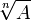
\includegraphics[scale=.6]{graphics/4518ae089727239af6a569824b9b86e2.png}
of a positive real number \emph{A}, as explained at the
\href{http://en.wikipedia.org/wiki/Nth\_root\_algorithm}{Wikipedia
page}.

\begin{wideverbatim}

(load "@lib/math.l")

(de nthroot (N A)
   (let (X1 A  X2 (*/ A N))
      (until (= X1 X2)
         (setq
            X1 X2
            X2 (*/
               (+
                  (* X1 (dec N))
                  (*/ A 1.0 (pow X1 (* (dec N) 1.0))) )
               N ) ) )
      X2 ) )

(prinl (format (nthroot 2  2.0) *Scl))
(prinl (format (nthroot 3 12.3) *Scl))
(prinl (format (nthroot 4 45.6) *Scl))

Output:

1.414214
2.308350
2.598611

\end{wideverbatim}

\pagebreak{}
\section*{Number names}

Show how to spell out a number in English. You can use a preexisting
implementation or roll your own, but you should support inputs up to at
least one million (or the maximum value of your language's default
bounded integer type, if that's less). Support for inputs other than
positive integers (like zero, negative integers, and floating-point
numbers) is optional.


\begin{wideverbatim}

(de numName (N)
   (cond
      ((=0 N) "zero")
      ((lt0 N) (pack "minus " (numName (- N))))
      (T (numNm N)) ) )


(de numNm (N)
   (cond
      ((=0 N))
      ((> 14 N)
         (get '("one" "two" "three" "four" "five" "six" "seven" "eight"
                  "nine" "ten" "eleven" "twelve" "thirteen" ) N ) )
      ((= 15 N) "fifteen")
      ((= 18 N) "eighteen")
      ((> 20 N) (pack (numNm (\% N 10)) "teen"))
      ((> 100 N)
         (pack
            (get '("twen" "thir" "for" "fif" "six" "seven" "eigh" "nine") (dec (/ N 10)))
            "ty"
            (unless (=0 (\% N 10))
               (pack "-" (numNm (\% N 10))) ) ) )
      ((rank N '((100 . "hundred") (1000 . "thousand") (1000000 . "million")))
         (pack (numNm (/ N (car @))) " " (cdr @) " " (numNm (\% N (car @)))) ) ) )

\end{wideverbatim}

\pagebreak{}
\section*{Number reversal game}

Given a jumbled list of the numbers 1 to 9 that are definitely
\emph{not} in ascending order, show the list then ask the player how
many digits from the left to reverse. Reverse those digits, then ask
again, until all the digits end up in ascending order.

The score is the count of the reversals needed to attain the ascending
order.

Note: Assume the players input does not need extra validation.

C.f: \emph{Sorting algorithms/Pancake sort},
\href{http://en.wikipedia.org/wiki/Pancake\_sorting}{Pancake sorting}.


\begin{wideverbatim}

(load "@lib/simul.l")

(de reversalGame ()
   (let (Lst (shuffle (range 1 9))  Cnt 0)
      (while (apply < Lst)
         (setq Lst (shuffle Lst)) )
      (loop
         (printsp Lst)
         (T (apply < Lst) Cnt)
         (NIL (num? (read)))
         (setq Lst (flip Lst @))
         (inc 'Cnt) ) ) )

Output:

: (reversalGame)
(1 7 6 8 4 2 3 5 9) 4
(8 6 7 1 4 2 3 5 9) 8
(5 3 2 4 1 7 6 8 9) 6
(7 1 4 2 3 5 6 8 9) 7
(6 5 3 2 4 1 7 8 9) 6
(1 4 2 3 5 6 7 8 9) 2
(4 1 2 3 5 6 7 8 9) 4
(3 2 1 4 5 6 7 8 9) 3
(1 2 3 4 5 6 7 8 9) -> 8

\end{wideverbatim}

\pagebreak{}
\section*{Numeric error propagation}


If f, a, and b are values with uncertainties $\sigma$\textsubscript{f},
$\sigma$\textsubscript{a}, and $\sigma$\textsubscript{b}. and c is a constant; then if
f is derived from a, b, and c in the following ways, then
$\sigma$\textsubscript{f} can be calculated as follows:

Addition/Subtraction

\begin{itemize}
\item
  If f = a ± c, or f = c ± a then \textbf{$\sigma$\textsubscript{f} =
  $\sigma$\textsubscript{a}}
\item
  If f = a ± b then \textbf{$\sigma$\textsubscript{f}\textsuperscript{2} =
  $\sigma$\textsubscript{a}\textsuperscript{2} +
  $\sigma$\textsubscript{b}\textsuperscript{2}}
\end{itemize}

Multiplication/Division

\begin{itemize}
\item
  If f = ca or f = ac then \textbf{$\sigma$\textsubscript{f} =
  \textbar{}c$\sigma$\textsubscript{a}\textbar{}}
\item
  If f = ab or f = a / b then
  \textbf{$\sigma$\textsubscript{f}\textsuperscript{2} = f\textsuperscript{2}(
  ($\sigma$\textsubscript{a} / a)\textsuperscript{2} + ($\sigma$\textsubscript{b} /
  b)\textsuperscript{2})}
\end{itemize}

Exponentiation

\begin{itemize}
\item
  If f = a\textsuperscript{c} then \textbf{$\sigma$\textsubscript{f} =
  \textbar{}fc($\sigma$\textsubscript{a} / a)\textbar{}}
\end{itemize}

Caution:

This implementation of error propagation does not address issues of
dependent and independent values. It is assumed that a and b are
independent and so the formula for multiplication should not be applied
to a*a for exam{[}ple. See
\emph{the talk page} for some of
the implications of this issue.

\pagebreak{}

\begin{description}
\item[Task details]
\end{description}

\begin{enumerate}
\item
  Add an uncertain number type to your language that can support
  addition, subtraction, multiplication, division, and exponentiation
  between numbers with an associated error term together with `normal'
  floating point numbers without an associated error term. \\Implement
  enough functionality to perform the following calculations.
\item
  Given coordinates and their errors:\\x1 = 100 ± 1.1\\y1 = 50 ± 1.2\\x2
  = 200 ± 2.2\\y2 = 100 ± 2.3\\ if point p1 is located at (x1, y1) and
  p2 is at (x2, y2); calculate the distance between the two points using
  the classic pythagorean formula:\\ \textbf{d = √((x1 -
  x2)\textsuperscript{2} + (y1 - y2)\textsuperscript{2})}
\item
  Print and display both \textbf{d} and its error.
\end{enumerate}

\begin{description}
\item[References]
\end{description}

\begin{itemize}
\item
  \href{http://casa.colorado.edu/~benderan/teaching/astr3510/stats.pdf}{A
  Guide to Error Propagation} B. Keeney, 2005.
\item
  \href{http://en.wikipedia.org/wiki/Propagation\_of\_uncertainty}{Propagation
  of uncertainty} Wikipedia.
\end{itemize}

\begin{description}
\item[Cf.]
\end{description}

\begin{itemize}
\item
  \emph{Quaternion type}
\end{itemize}


\begin{wideverbatim}

For this task, we overload the built-in arithmetic functions. If the arguments
are cons pairs, they are assumed to hold the fixpoint number in the CAR, and the
uncertainty's square in the CDR. Otherwise normal numbers are handled as usual.

The overloaded +, -, * and / operators look a bit complicated, because they must
handle an arbitrary number of arguments to be compatible with the standard
operators.

(scl 12)
(load "@lib/math.l")

# Overload arithmetic operators +, -, *, / and **
(redef + @
   (let R (next)
      (while (args)
         (let N (next)
            (setq R
               (if2 (atom R) (atom N)
                  (+ R N)                       # c + c
                  (cons (+ R (car N)) (cdr N))  # c + a
                  (cons (+ (car R) N) (cdr R))  # a + c
                  (cons                         # a + b
                     (+ (car R) (car N))
                     (+ (cdr R) (cdr N)) ) ) ) ) )
      R ) )

(redef - @
   (let R (next)
      (ifn (args)
         (- R)
         (while (args)
            (let N (next)
               (setq R
                  (if2 (atom R) (atom N)
                     (- R N)                       # c - c
                     (cons (- R (car N)) (cdr N))  # c - a
                     (cons (- (car R) N) (cdr R))  # a - c
                     (cons                         # a - b
                        (- (car R) (car N))
                        (+ (cdr R) (cdr N)) ) ) ) ) )
         R ) ) )


\end{wideverbatim}

\begin{wideverbatim}


(redef * @
   (let R (next)
      (while (args)
         (let N (next)
            (setq R
               (if2 (atom R) (atom N)
                  (* R N)                                        # c * c
                  (cons                                          # c * a
                     (*/ R (car N) 1.0)
                     (mul2div2 (cdr N) R 1.0) )
                  (cons                                          # a * c
                     (*/ (car R) N 1.0)
                     (mul2div2 (cdr R) N 1.0) )
                  (uncMul (*/ (car R) (car N) 1.0) R N) ) ) ) )  # a * b
      R ) )

(redef / @
   (let R (next)
      (while (args)
         (let N (next)
            (setq R
               (if2 (atom R) (atom N)
                  (/ R N)                                        # c / c
                  (cons                                          # c / a
                     (*/ R 1.0 (car N))
                     (mul2div2 (cdr N) R 1.0) )
                  (cons                                          # a / c
                     (*/ (car R) 1.0 N)
                     (mul2div2 (cdr R) N 1.0) )
                  (uncMul (*/ (car R) 1.0 (car N)) R N) ) ) ) )  # a / b
      R ) )

(redef ** (A C)
   (if (atom A)
      (** A C)
      (let F (pow (car A) C)
         (cons F
            (mul2div2 (cdr A) (*/ F C (car A)) 1.0) ) ) ) )

\end{wideverbatim}

\begin{wideverbatim}


# Utilities
(de mul2div2 (A B C)
   (*/ A B B (* C C)) )

(de uncMul (F R N)
   (cons F
      (mul2div2
         (+
            (mul2div2 (cdr R) 1.0 (car R))
            (mul2div2 (cdr N) 1.0 (car N)) )
         F
         1.0 ) ) )

# I/O conversion
(de unc (N U)
   (if U
      (cons N (*/ U U 1.0))
      (pack
         (round (car N) 10)
         " ± "
         (round (sqrt (* 1.0 (cdr N))) 8) ) ) )

Test:

(de distance (X1 Y1 X2 Y2)
   (**
      (+ (** (- X1 X2) 2.0) (** (- Y1 Y2) 2.0))
      0.5 ) )

(prinl "Distance: "
   (unc
      (distance
         (unc 100. 1.1)
         (unc 50. 1.2)
         (unc 200. 2.2)
         (unc 100. 2.3) ) ) )

Output:

Distance: 111.8033988750 ± 2.48716706

\end{wideverbatim}

\pagebreak{}
\section*{Numerical integration}

Write functions to calculate the definite integral of a function
(\emph{f(x)}) using
\href{http://en.wikipedia.org/wiki/Rectangle\_method}{rectangular}
(left, right, and midpoint),
\href{http://en.wikipedia.org/wiki/Trapezoidal\_rule}{trapezium}, and
\href{http://en.wikipedia.org/wiki/Simpson\%27s\_rule}{Simpson's}
methods. Your functions should take in the upper and lower bounds
(\emph{a} and \emph{b}) and the number of approximations to make in that
range (\emph{n}). Assume that your example already has a function that
gives values for \emph{f(x)}.

Simpson's method is defined by the following pseudocode:

\begin{verbatim}
h := (b - a) / n
sum1 := f(a + h/2)
sum2 := 0

loop on i from 1 to (n - 1)
    sum1 := sum1 + f(a + h * i + h/2)
    sum2 := sum2 + f(a + h * i)

answer := (h / 6) * (f(a) + f(b) + 4*sum1 + 2*sum2)
\end{verbatim}

Demonstrate your function by showing the results for:

\begin{itemize}
\item
  f(x) = x\^{}3, where x is {[}0,1{]}, with 100 approximations. The
  exact result is 1/4, or 0.25.
\item
  f(x) = 1/x, where x is {[}1,100{]}, with 1,000 approximations. The
  exact result is the natural log of 100, or about 4.605170
\item
  f(x) = x, where x is {[}0,5000{]}, with 5,000,000 approximations. The
  exact result is 12,500,000.
\item
  f(x) = x, where x is {[}0,6000{]}, with 6,000,000 approximations. The
  exact result is 18,000,000.
\end{itemize}

\textbf{See also}

\begin{itemize}
\item
  \emph{Active object} for integrating a function
  of real time.
\item
  \emph{Numerical
  integration/Gauss-Legendre Quadrature} for another integration method.
\end{itemize}



\begin{wideverbatim}

(scl 6)

(de leftRect (Fun X)
   (Fun X) )

(de rightRect (Fun X H)
   (Fun (+ X H)) )

(de midRect (Fun X H)
   (Fun (+ X (/ H 2))) )

(de trapezium (Fun X H)
   (/ (+ (Fun X) (Fun (+ X H))) 2) )

(de simpson (Fun X H)
   (*/
      (+
         (Fun X)
         (* 4 (Fun (+ X (/ H 2))))
         (Fun (+ X H)) )
      6 ) )

(de square (X)
   (*/ X X 1.0) )

(de integrate (Fun From To Steps Meth)
   (let (H (/ (- To From) Steps)  Sum 0)
      (for (X From  (>= (- To H) X)  (+ X H))
         (inc 'Sum (Meth Fun X H)) )
      (*/ H Sum 1.0) ) )

(prinl (round (integrate square 3.0 7.0 30 simpson)))

Output:

105.333

\end{wideverbatim}



% %%%%%%%%%%%%%%%%%%%%%%%% referenc.tex %%%%%%%%%%%%%%%%%%%%%%%%%%%%%%
% sample references
% %
% Use this file as a template for your own input.
%
%%%%%%%%%%%%%%%%%%%%%%%% Springer-Verlag %%%%%%%%%%%%%%%%%%%%%%%%%%
%
% BibTeX users please use
% \bibliographystyle{}
% \bibliography{}
%
\biblstarthook{In view of the parallel print and (chapter-wise) online publication of your book at \url{www.springerlink.com} it has been decided that -- as a genreral rule --  references should be sorted chapter-wise and placed at the end of the individual chapters. However, upon agreement with your contact at Springer you may list your references in a single seperate chapter at the end of your book. Deactivate the class option \texttt{sectrefs} and the \texttt{thebibliography} environment will be put out as a chapter of its own.\\\indent
References may be \textit{cited} in the text either by number (preferred) or by author/year.\footnote{Make sure that all references from the list are cited in the text. Those not cited should be moved to a separate \textit{Further Reading} section or chapter.} The reference list should ideally be \textit{sorted} in alphabetical order -- even if reference numbers are used for the their citation in the text. If there are several works by the same author, the following order should be used: 
\begin{enumerate}
\item all works by the author alone, ordered chronologically by year of publication
\item all works by the author with a coauthor, ordered alphabetically by coauthor
\item all works by the author with several coauthors, ordered chronologically by year of publication.
\end{enumerate}
The \textit{styling} of references\footnote{Always use the standard abbreviation of a journal's name according to the ISSN \textit{List of Title Word Abbreviations}, see \url{http://www.issn.org/en/node/344}} depends on the subject of your book:
\begin{itemize}
\item The \textit{two} recommended styles for references in books on \textit{mathematical, physical, statistical and computer sciences} are depicted in ~\cite{science-contrib, science-online, science-mono, science-journal, science-DOI} and ~\cite{phys-online, phys-mono, phys-journal, phys-DOI, phys-contrib}.
\item Examples of the most commonly used reference style in books on \textit{Psychology, Social Sciences} are~\cite{psysoc-mono, psysoc-online,psysoc-journal, psysoc-contrib, psysoc-DOI}.
\item Examples for references in books on \textit{Humanities, Linguistics, Philosophy} are~\cite{humlinphil-journal, humlinphil-contrib, humlinphil-mono, humlinphil-online, humlinphil-DOI}.
\item Examples of the basic Springer style used in publications on a wide range of subjects such as \textit{Computer Science, Economics, Engineering, Geosciences, Life Sciences, Medicine, Biomedicine} are ~\cite{basic-contrib, basic-online, basic-journal, basic-DOI, basic-mono}. 
\end{itemize}
}

\begin{thebibliography}{99.}%
% and use \bibitem to create references.
%
% Use the following syntax and markup for your references if 
% the subject of your book is from the field 
% "Mathematics, Physics, Statistics, Computer Science"
%
% Contribution 
\bibitem{science-contrib} Broy, M.: Software engineering --- from auxiliary to key technologies. In: Broy, M., Dener, E. (eds.) Software Pioneers, pp. 10-13. Springer, Heidelberg (2002)
%
% Online Document
\bibitem{science-online} Dod, J.: Effective substances. In: The Dictionary of Substances and Their Effects. Royal Society of Chemistry (1999) Available via DIALOG. \\
\url{http://www.rsc.org/dose/title of subordinate document. Cited 15 Jan 1999}
%
% Monograph
\bibitem{science-mono} Geddes, K.O., Czapor, S.R., Labahn, G.: Algorithms for Computer Algebra. Kluwer, Boston (1992) 
%
% Journal article
\bibitem{science-journal} Hamburger, C.: Quasimonotonicity, regularity and duality for nonlinear systems of partial differential equations. Ann. Mat. Pura. Appl. \textbf{169}, 321--354 (1995)
%
% Journal article by DOI
\bibitem{science-DOI} Slifka, M.K., Whitton, J.L.: Clinical implications of dysregulated cytokine production. J. Mol. Med. (2000) doi: 10.1007/s001090000086 
%
\bigskip

% Use the following (APS) syntax and markup for your references if 
% the subject of your book is from the field 
% "Mathematics, Physics, Statistics, Computer Science"
%
% Online Document
\bibitem{phys-online} J. Dod, in \textit{The Dictionary of Substances and Their Effects}, Royal Society of Chemistry. (Available via DIALOG, 1999), 
\url{http://www.rsc.org/dose/title of subordinate document. Cited 15 Jan 1999}
%
% Monograph
\bibitem{phys-mono} H. Ibach, H. L\"uth, \textit{Solid-State Physics}, 2nd edn. (Springer, New York, 1996), pp. 45-56 
%
% Journal article
\bibitem{phys-journal} S. Preuss, A. Demchuk Jr., M. Stuke, Appl. Phys. A \textbf{61}
%
% Journal article by DOI
\bibitem{phys-DOI} M.K. Slifka, J.L. Whitton, J. Mol. Med., doi: 10.1007/s001090000086
%
% Contribution 
\bibitem{phys-contrib} S.E. Smith, in \textit{Neuromuscular Junction}, ed. by E. Zaimis. Handbook of Experimental Pharmacology, vol 42 (Springer, Heidelberg, 1976), p. 593
%
\bigskip
%
% Use the following syntax and markup for your references if 
% the subject of your book is from the field 
% "Psychology, Social Sciences"
%
%
% Monograph
\bibitem{psysoc-mono} Calfee, R.~C., \& Valencia, R.~R. (1991). \textit{APA guide to preparing manuscripts for journal publication.} Washington, DC: American Psychological Association.
%
% Online Document
\bibitem{psysoc-online} Dod, J. (1999). Effective substances. In: The dictionary of substances and their effects. Royal Society of Chemistry. Available via DIALOG. \\
\url{http://www.rsc.org/dose/Effective substances.} Cited 15 Jan 1999.
%
% Journal article
\bibitem{psysoc-journal} Harris, M., Karper, E., Stacks, G., Hoffman, D., DeNiro, R., Cruz, P., et al. (2001). Writing labs and the Hollywood connection. \textit{J Film} Writing, 44(3), 213--245.
%
% Contribution 
\bibitem{psysoc-contrib} O'Neil, J.~M., \& Egan, J. (1992). Men's and women's gender role journeys: Metaphor for healing, transition, and transformation. In B.~R. Wainrig (Ed.), \textit{Gender issues across the life cycle} (pp. 107--123). New York: Springer.
%
% Journal article by DOI
\bibitem{psysoc-DOI}Kreger, M., Brindis, C.D., Manuel, D.M., Sassoubre, L. (2007). Lessons learned in systems change initiatives: benchmarks and indicators. \textit{American Journal of Community Psychology}, doi: 10.1007/s10464-007-9108-14.
%
%
% Use the following syntax and markup for your references if 
% the subject of your book is from the field 
% "Humanities, Linguistics, Philosophy"
%
\bigskip
%
% Journal article
\bibitem{humlinphil-journal} Alber John, Daniel C. O'Connell, and Sabine Kowal. 2002. Personal perspective in TV interviews. \textit{Pragmatics} 12:257--271
%
% Contribution 
\bibitem{humlinphil-contrib} Cameron, Deborah. 1997. Theoretical debates in feminist linguistics: Questions of sex and gender. In \textit{Gender and discourse}, ed. Ruth Wodak, 99--119. London: Sage Publications.
%
% Monograph
\bibitem{humlinphil-mono} Cameron, Deborah. 1985. \textit{Feminism and linguistic theory.} New York: St. Martin's Press.
%
% Online Document
\bibitem{humlinphil-online} Dod, Jake. 1999. Effective substances. In: The dictionary of substances and their effects. Royal Society of Chemistry. Available via DIALOG. \\
http://www.rsc.org/dose/title of subordinate document. Cited 15 Jan 1999
%
% Journal article by DOI
\bibitem{humlinphil-DOI} Suleiman, Camelia, Daniel C. O�Connell, and Sabine Kowal. 2002. `If you and I, if we, in this later day, lose that sacred fire...�': Perspective in political interviews. \textit{Journal of Psycholinguistic Research}. doi: 10.1023/A:1015592129296.
%
%
%
\bigskip
%
%
% Use the following syntax and markup for your references if 
% the subject of your book is from the field 
% "Computer Science, Economics, Engineering, Geosciences, Life Sciences"
%
%
% Contribution 
\bibitem{basic-contrib} Brown B, Aaron M (2001) The politics of nature. In: Smith J (ed) The rise of modern genomics, 3rd edn. Wiley, New York 
%
% Online Document
\bibitem{basic-online} Dod J (1999) Effective Substances. In: The dictionary of substances and their effects. Royal Society of Chemistry. Available via DIALOG. \\
\url{http://www.rsc.org/dose/title of subordinate document. Cited 15 Jan 1999}
%
% Journal article by DOI
\bibitem{basic-DOI} Slifka MK, Whitton JL (2000) Clinical implications of dysregulated cytokine production. J Mol Med, doi: 10.1007/s001090000086
%
% Journal article
\bibitem{basic-journal} Smith J, Jones M Jr, Houghton L et al (1999) Future of health insurance. N Engl J Med 965:325--329
%
% Monograph
\bibitem{basic-mono} South J, Blass B (2001) The future of modern genomics. Blackwell, London 
%
\end{thebibliography}

